\documentclass[12pt,a4paper]{report}
\usepackage{tbu_report}

% ==============================================================================
% NẠP THÔNG TIN BÁO CÁO (Chỉnh sửa thông tin tại file thongtinbia.tex)
% ==============================================================================
% ==============================================================================
% THÔNG TIN BÁO CÁO / KHÓA LUẬN / ĐỀ TÀI NCKH
% Chỉnh sửa thông tin tại file này, hệ thống sẽ tự động cập nhật vào trang bìa
% ==============================================================================

% 1. Thông tin đơn vị đào tạo
\ministry{BỘ GIÁO DỤC VÀ ĐÀO TẠO}
\university{TRƯỜNG ĐẠI HỌC TÂY BẮC}
\faculty{KHOA TỰ NHIÊN VÀ CÔNG NGHỆ THÔNG TIN}

% 2. Thông tin loại báo cáo và tên đề tài
\reporttype{BÁO CÁO TỔNG KẾT}
\reportsubtype{ĐỀ TÀI NGHIÊN CỨU KHOA HỌC CỦA SINH VIÊN}
\title{NGHIÊN CỨU CÁC THUẬT TOÁN GẦN ĐÚNG GIẢI CÁC BÀI TOÁN s-CLUB}
\scientificfield{Công nghệ Thông tin}

% 3. Thông tin lớp, ngành, khóa học
\courseclass{K64 ĐẠI HỌC CNTT}
\academicyear{4/Số năm đào tạo: 4}
\major{Công nghệ Thông tin}

% 4. Thông tin người hướng dẫn và sinh viên chịu trách nhiệm chính
\leadstudent{Lò Mạnh Đạt}
\advisor{TS. Phạm Đình Thành}

% 5. Địa điểm và thời gian báo cáo
\location{Sơn La}
\reportdate{tháng 5 năm 2026}

% 6. Đường dẫn logo trường
\logopath{tbu_logo.png}

% 7. Danh sách Sinh viên thực hiện: \addstudent{Họ và tên}{Giới tính}{Dân tộc}
\addstudent{Lò Mạnh Đạt}{Nam}{Thái}
\addstudent{Phạm Thị Thanh Hảo}{Nữ}{Kinh}
\addstudent{Tòng Lưu Anh Tú}{Nam}{Thái}
\addstudent{Nguyễn Huy Hoàng}{Nam}{Kinh}


\begin{document}

% ==============================================================================
% 1. TRANG BÌA CHÍNH (BÌA NGOÀI) VÀ TRANG BÌA PHỤ
% ==============================================================================
\makeoutercover
\makeinnercover

% ==============================================================================
% 2. LỜI CAM ĐOAN VÀ LỜI CẢM ƠN
% ==============================================================================
\cleardoublepage
\pagenumbering{roman}
% !TEX root = ../main.tex
\begin{pledge}
  Chúng tôi xin khẳng định rằng đây là công trình nghiên cứu của nhóm. Mọi số liệu và nguồn tham khảo đều trung thực, chính xác và được trích dẫn đầy đủ. Chúng tôi hoàn toàn chịu trách nhiệm về lời cam đoan này.
\end{pledge}

% !TEX root = ../main.tex
\begin{acknowledgements}
  Chúng tôi xin gửi lời cảm ơn chân thành và sâu sắc nhất đến các thầy cô giáo trong Khoa Công nghệ Thông tin - Trường Đại học Tây Bắc đã tận tình giảng dạy, hướng dẫn và tạo điều kiện thuận lợi cho nhóm chúng tôi trong suốt quá trình học tập và nghiên cứu.

  Đặc biệt, nhóm xin bày tỏ lòng biết ơn sâu sắc đến thầy \textbf{TS. Phạm Quốc Thắng} đã dành nhiều thời gian quý báu để định hướng, tận tình chỉ dẫn và đóng góp những ý kiến quý báu giúp nhóm hoàn thành tốt đề tài này.

  Dù đã có nhiều cố gắng, song bài báo cáo khó tránh khỏi những thiếu sót. Nhóm kính mong nhận được sự góp ý chân thành từ quý thầy cô và các bạn để đề tài được hoàn thiện hơn.

  Xin chân thành cảm ơn!
\end{acknowledgements}


% ==============================================================================
% 3. MỤC LỤC VÀ CÁC DANH MỤC (HÌNH ẢNH, BẢNG BIỂU, TỪ VIẾT TẮT)
% ==============================================================================
\makecontentlists
\makelistoffigures
\makelistoftables
% !TEX root = ../main.tex
\begin{abbreviations}
  CNTT & Công nghệ Thông tin \\ \hline
  CSDL & Cơ sở dữ liệu \\ \hline
  GVHD & Giảng viên hướng dẫn \\ \hline
  NCKH & Nghiên cứu Khoa học \\ \hline
  TBU  & Trường Đại học Tây Bắc \\ \hline
\end{abbreviations}


% ==============================================================================
% 4. NỘI DUNG CHÍNH CỦA BÁO CÁO
% ==============================================================================
\cleardoublepage
\pagenumbering{arabic}

% !TEX root = ../main.tex
\unchapter{MỞ ĐẦU}

\unsection{1.1}{Tổng quan về hệ thống đề xuất}
Trình bày nghiên cứu, tìm hiểu tổng quan về hệ thống đề xuất. Tại Việt Nam, trên thế giới đã nghiên cứu và có những sản phẩm nào tương tự. Đánh giá chất lượng các sản phẩm đang có hoặc đã biết.

\unsection{1.2}{Mục đích nghiên cứu}
Nêu mục đích nghiên cứu của đề tài bài tập lớn, giải quyết bài toán thực tế nào và đem lại giá trị ra sao cho người dùng.

\unsection{1.3}{Đối tượng và phạm vi nghiên cứu}
Nêu đối tượng và phạm vi nghiên cứu của bài tập.

\unsection{1.4}{Phương pháp nghiên cứu}
Nêu các phương pháp nghiên cứu đã được sử dụng như: thu thập dữ liệu, phân tích mô hình học máy, khảo sát thực tế...

\unsection{1.5}{Tổ chức thực hiện}
Trình bày cách thức tổ chức nghiên cứu và phân công nhiệm vụ chi tiết cho từng thành viên. Nhóm đã tiến hành họp bàn, thống nhất phân công nhiệm vụ phù hợp với năng lực và sở trường của từng cá nhân nhằm bảo đảm tiến độ và hiệu quả thực hiện đề tài.

% !TEX root = ../main.tex
\chapter{CƠ SỞ LÝ THUYẾT}

\section{Mục 1.1}
Trình bày tổng quan phần lý thuyết liên quan đến đề tài \cite{ref1}.

\section{Mục 1.2}
Nội dung chi tiết về các khái niệm cơ bản và thuật toán liên quan.

\section{Mục 1.3}
Phân tích sâu hơn các kỹ thuật áp dụng trong hệ thống \cite{ref2}.

\subsection{Mục 1.3.1}
Chi tiết về mô hình lý thuyết được lựa chọn.

% !TEX root = ../main.tex
\chapter{PHÂN TÍCH THIẾT KẾ HỆ THỐNG}

\section{Mục 2.1}
Mô tả kiến trúc tổng quan của hệ thống bài tập lớn.

\subsection{Mục 2.1.1}
Sơ đồ kiến trúc và luồng dữ liệu của ứng dụng.

\begin{figure}[htbp]
  \centering
  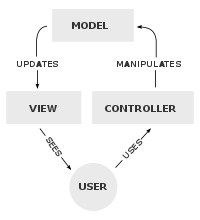
\includegraphics[width=0.6\textwidth]{sample_img.png}
  \caption{Hình ảnh mẫu sơ đồ hệ thống}
  \label{fig:sample}
\end{figure}

Như được thể hiện trên Hình \ref{fig:sample}, hệ thống gồm các thành phần cơ bản xử lý từ đầu vào đến kết quả trả về.

\subsection{Mục 2.1.2}
Phân tích thiết kế Cơ sở dữ liệu và các thành phần giao tiếp API.

% !TEX root = ../main.tex
\chapter{XÂY DỰNG VÀ KIỂM THỬ HỆ THỐNG}

\section{Mục 3.1}
Quá trình cài đặt và thực nghiệm hệ thống.

\begin{table}[htbp]
  \centering
  \caption{Bảng mẫu đánh giá kết quả thực nghiệm}
  \label{tab:sample}
  \begin{tabular}{|c|l|c|c|}
    \hline
    \textbf{STT} & \textbf{Tên tiêu chí}   & \textbf{Đơn vị} & \textbf{Kết quả} \\ \hline
    1            & Độ chính xác (Accuracy) & \%              & 94.5 \%          \\ \hline
    2            & Thời gian phản hồi      & giây            & 0.12 s           \\ \hline
    3            & Dung lượng bộ nhớ       & MB              & 45 MB            \\ \hline
  \end{tabular}
\end{table}

Bảng \ref{tab:sample} tổng hợp kết quả đo đạc các chỉ số hiệu năng của hệ thống.

\section{Mục 3.2}
Đánh giá mức độ hoàn thiện và khả năng đáp ứng yêu cầu bài toán.

% !TEX root = ../main.tex
\unchapter{KẾT LUẬN VÀ KIẾN NGHỊ}
Nêu kết luận cơ bản về những công việc đã thực hiện và hướng nghiên cứu cải tiến hệ thống đề xuất trong tương lai.


% ==============================================================================
% 5. TÀI LIỆU THAM KHẢO
% ==============================================================================
\cleardoublepage
\input{tailieuthamkhao.bib}

\end{document}
